% Appendix Template

\appendixpagenumbering % Restart numbering for each appendix

\chapter{Android SmartCanton Manager: User's Guide} % Main appendix title
\label{AppendixAndroidAppUserGuide} 

% ---------------------------------------------------------------------- %
\section{Login Activity}
% ---------------------------------------------------------------------- %
\begin{figure}[ht!]
    \centering
    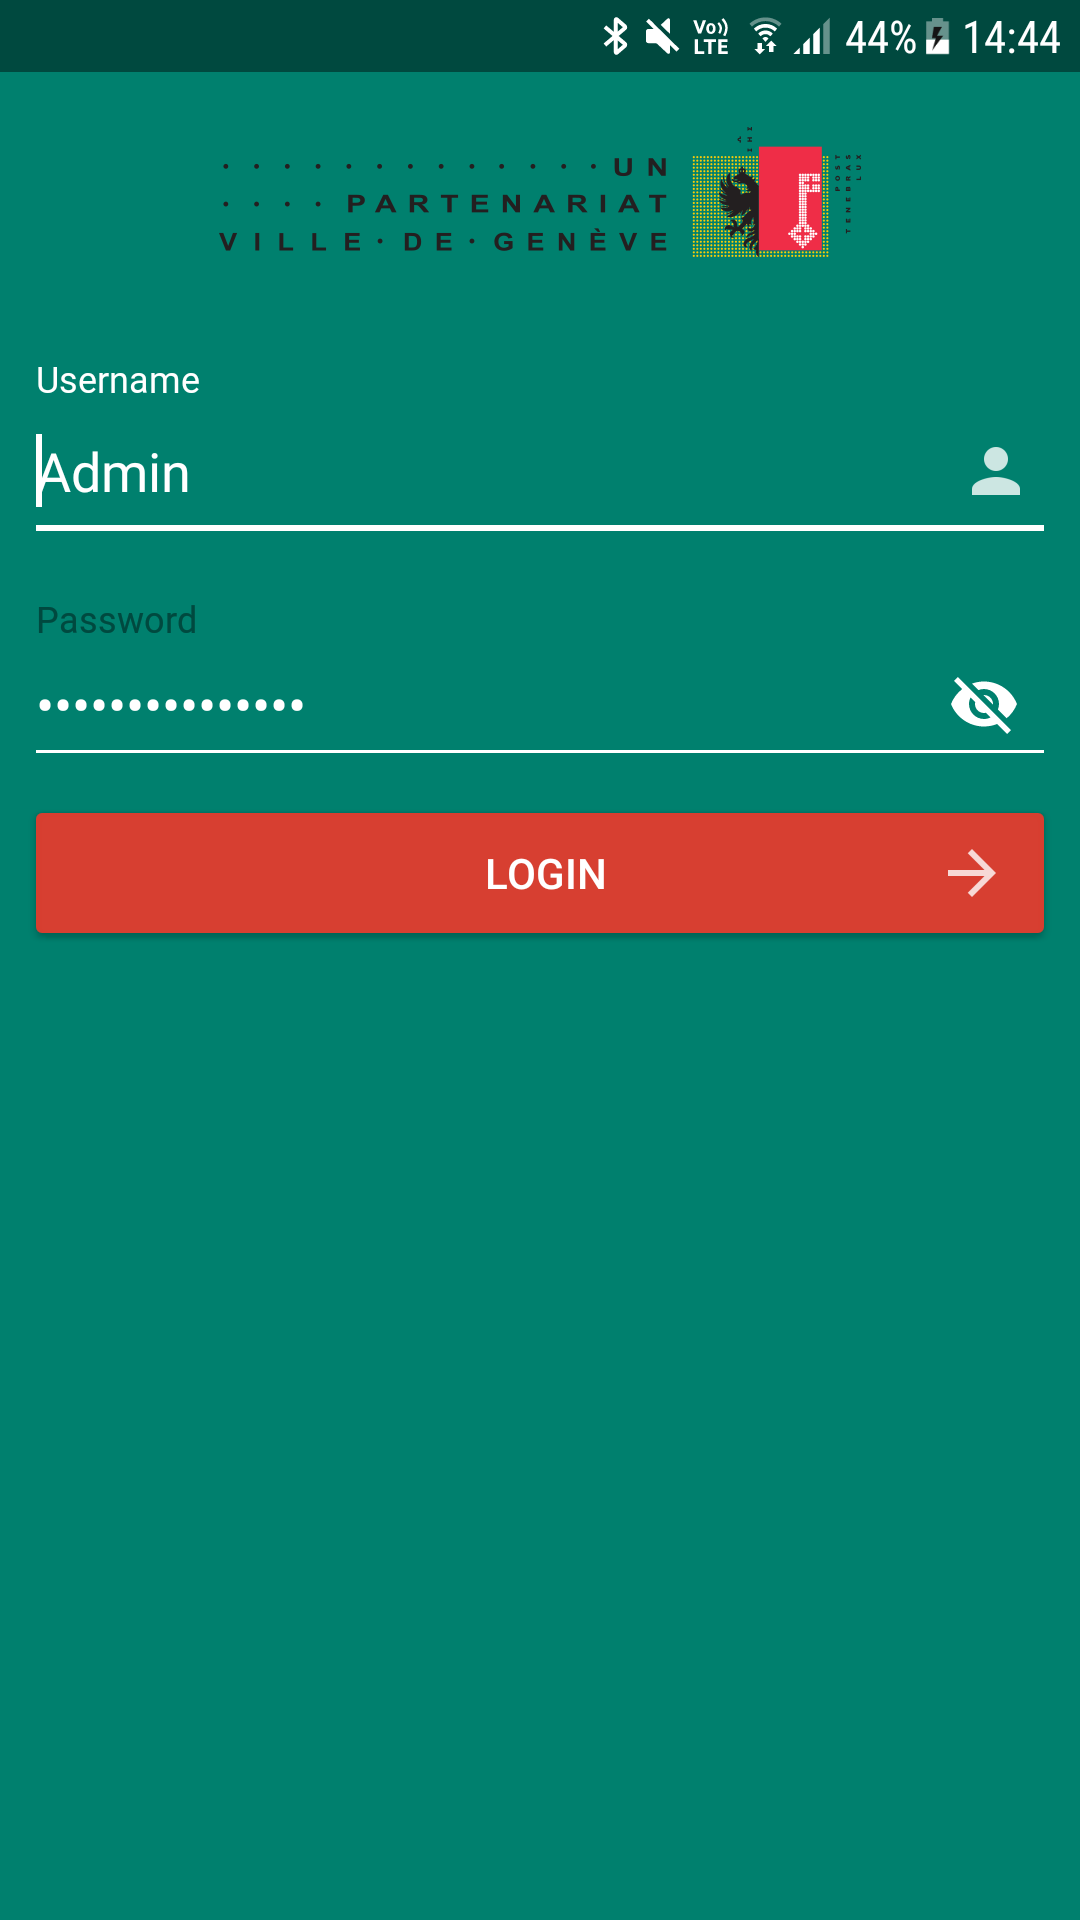
\includegraphics[width=0.33\textwidth]{Figures/Appendixes/Android/login_activity.png}
    \caption{SmartCanton Manager login activity}
    \label{fig_apdx-login_activity}
\end{figure}

When the application is launched, the user is required to log in using his credentials from the AppKey Server, as shown by the \cref{fig_apdx-login_activity}. 




% ---------------------------------------------------------------------- %
\FloatBarrier
\section{Bluetooth Activity : Scanner BLE Fragment}
% ---------------------------------------------------------------------- %
\begin{figure}[ht!]
    \centering
    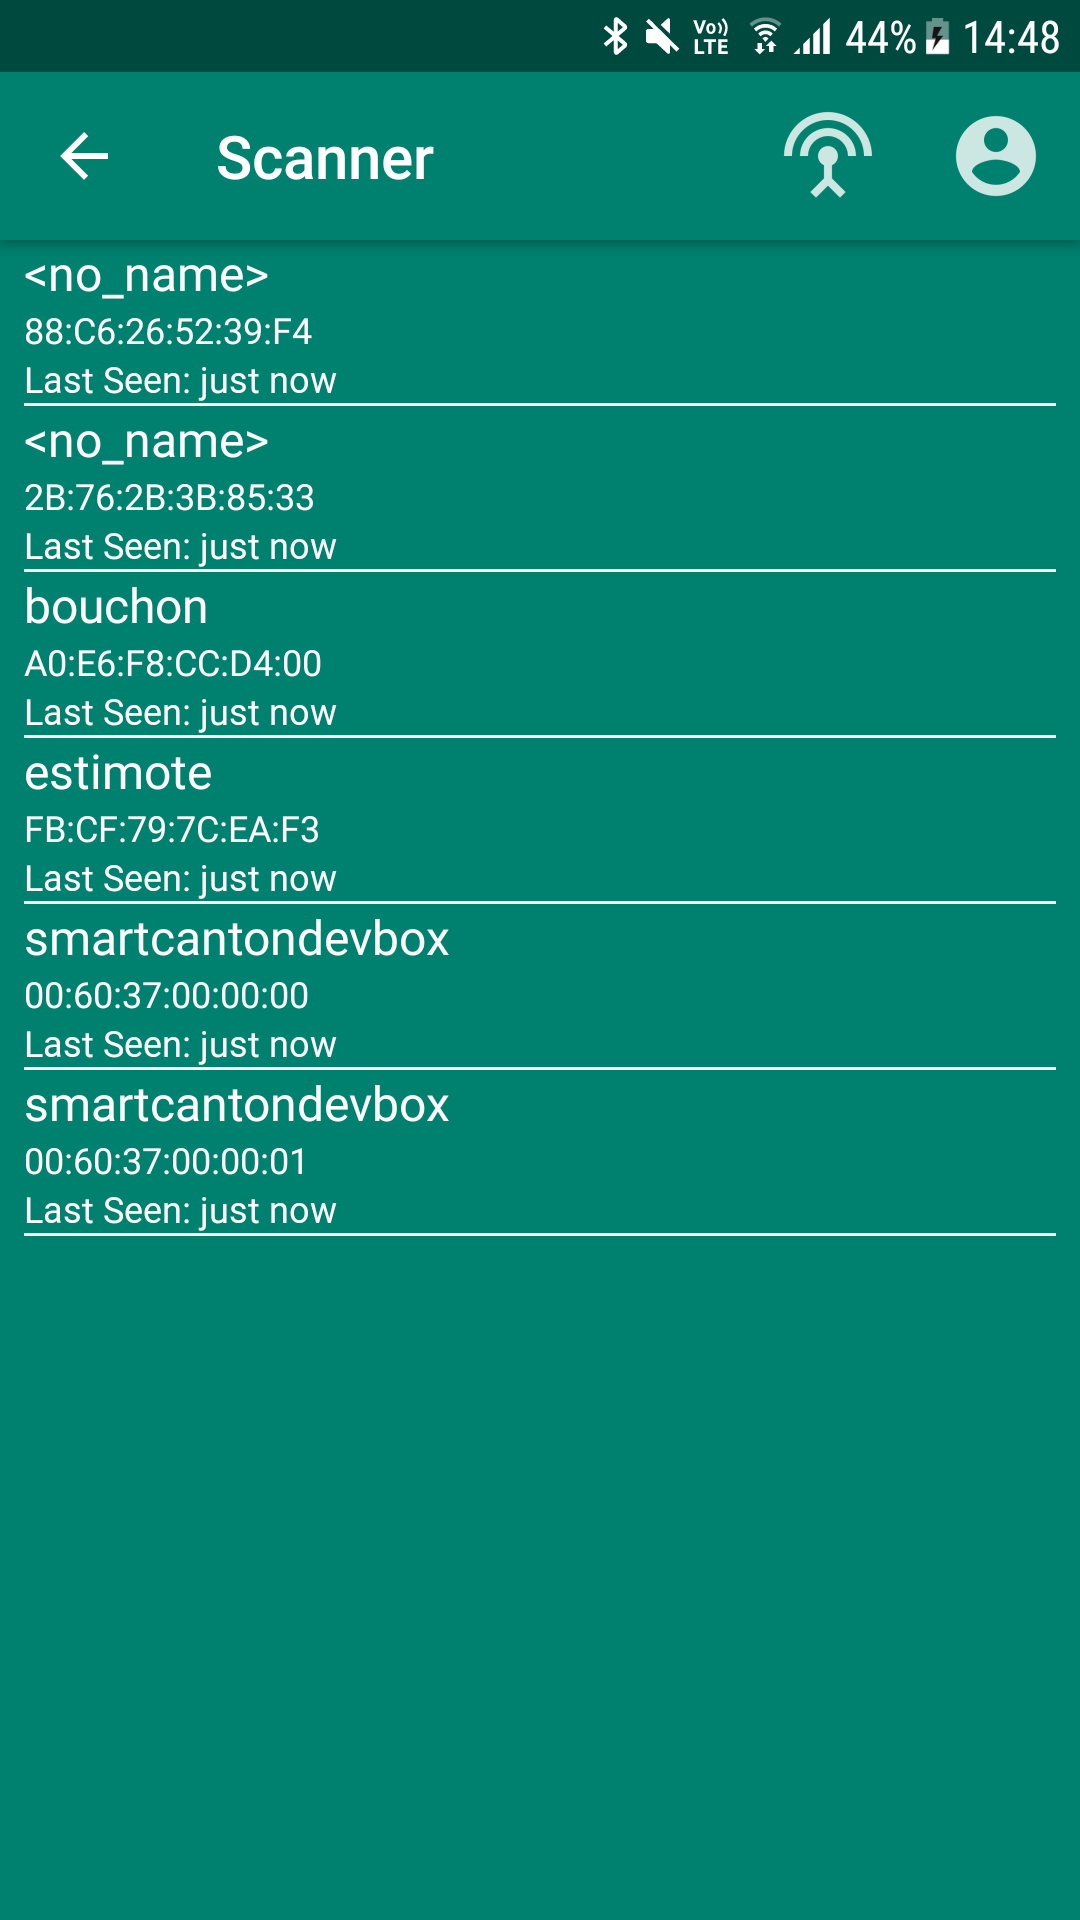
\includegraphics[width=0.33\textwidth]{Figures/Appendixes/Android/bluetooth_scanner_frag.png}
    \caption{SmartCanton Manager scanner fragment}
    \label{fig_apdx-bluetooth_scanner_frag}
\end{figure}

Once the user logged, all devices broadcasting ble packets nearby will be displayed in a list, as shown by the \cref{fig_apdx-bluetooth_scanner_frag}. The list can take a bit to be updated, just wait a moment. If the list still not display itself, just activate the \textit{airplane mode} on the phone and restart the SmartCanton Manager app.




% ---------------------------------------------------------------------- %
\FloatBarrier
\section{Bluetooth Activity : Device Management Fragment}
% ---------------------------------------------------------------------- %
\begin{figure}[ht!]
    \centering
    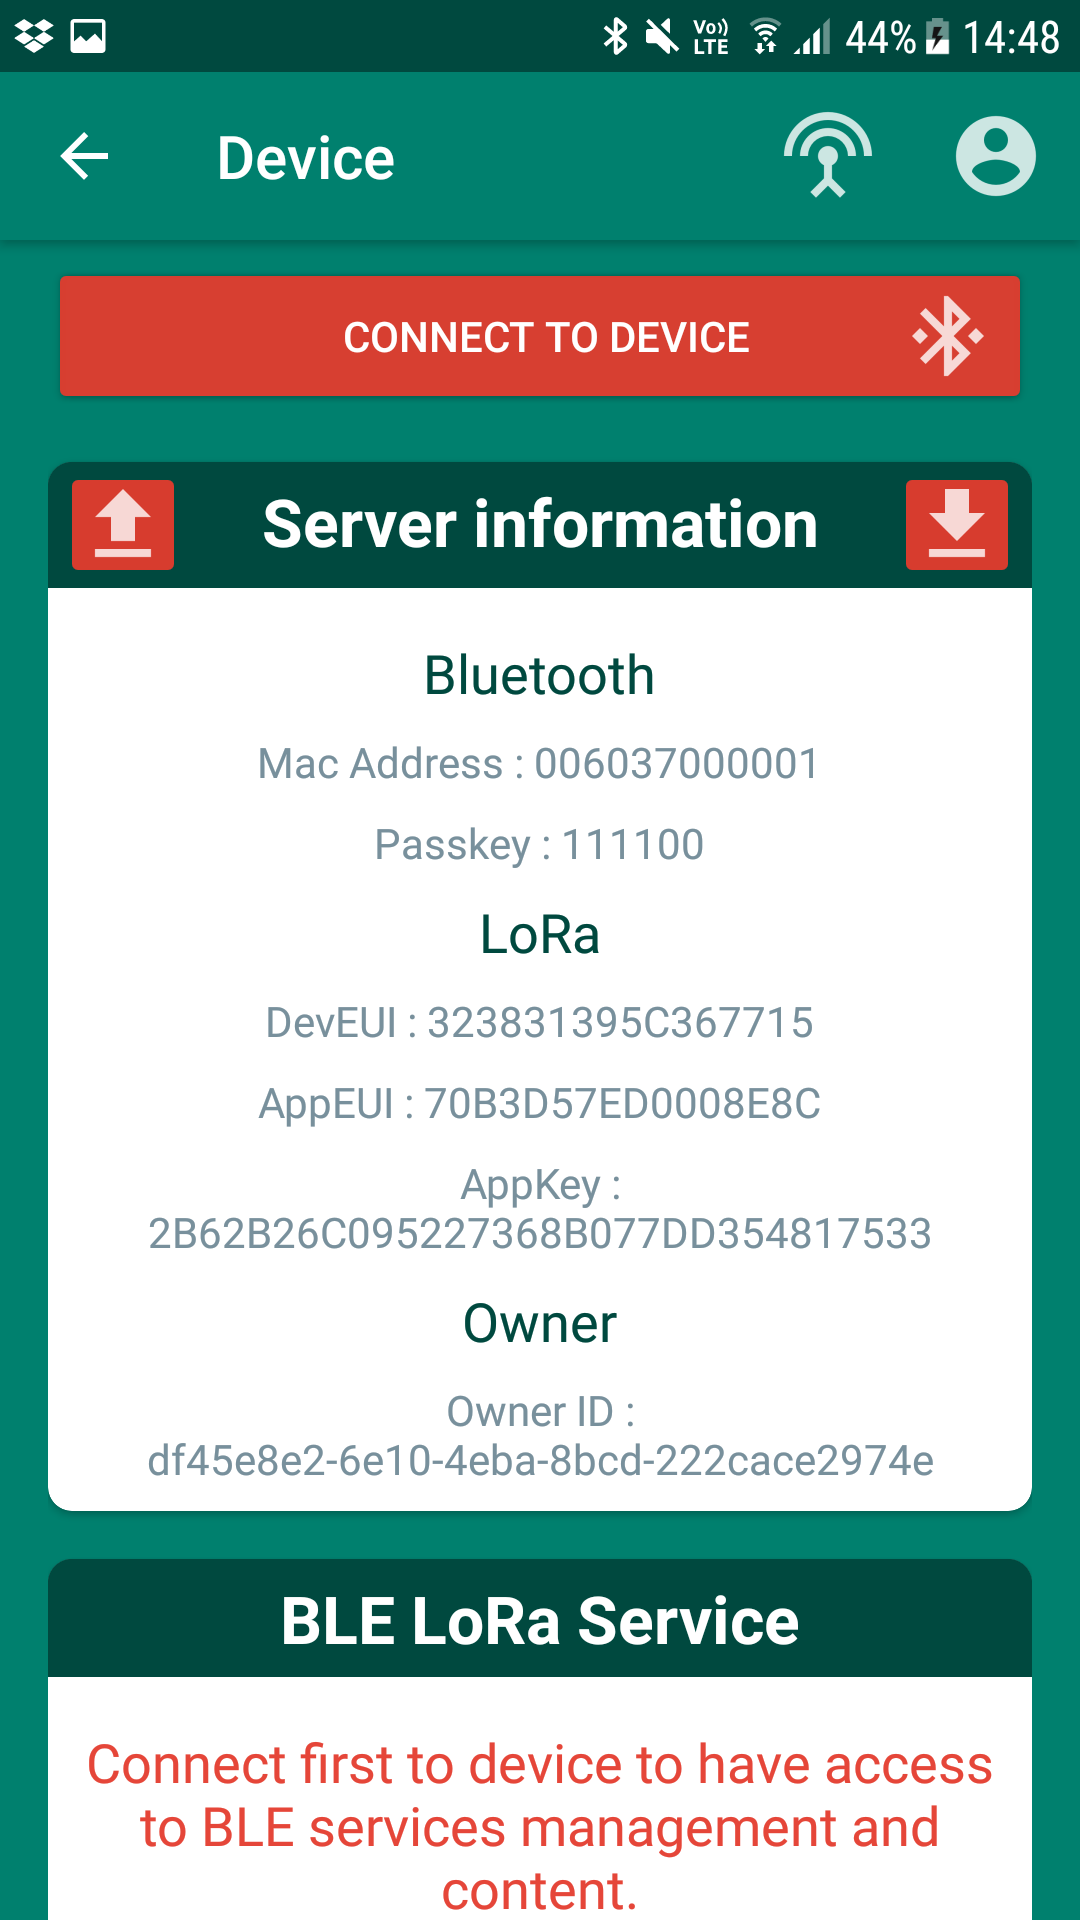
\includegraphics[width=0.33\textwidth]{Figures/Appendixes/Android/ble_dev_device_found.png}
    \caption{SmartCanton Manager device found on the server}
    \label{fig_apdx-ble_dev_device_found}
\end{figure}

When a Bluetooth device is selected on the BLE Scanner list, the fragment illustrated by the \cref{fig_apdx-ble_dev_device_found} is shown. If the device is found on the server, his information are displayed inside the \texttt{Server information} card. Those data can be updated by pressing the arrow on the right of the card.

\begin{figure}[ht!]
    \centering
    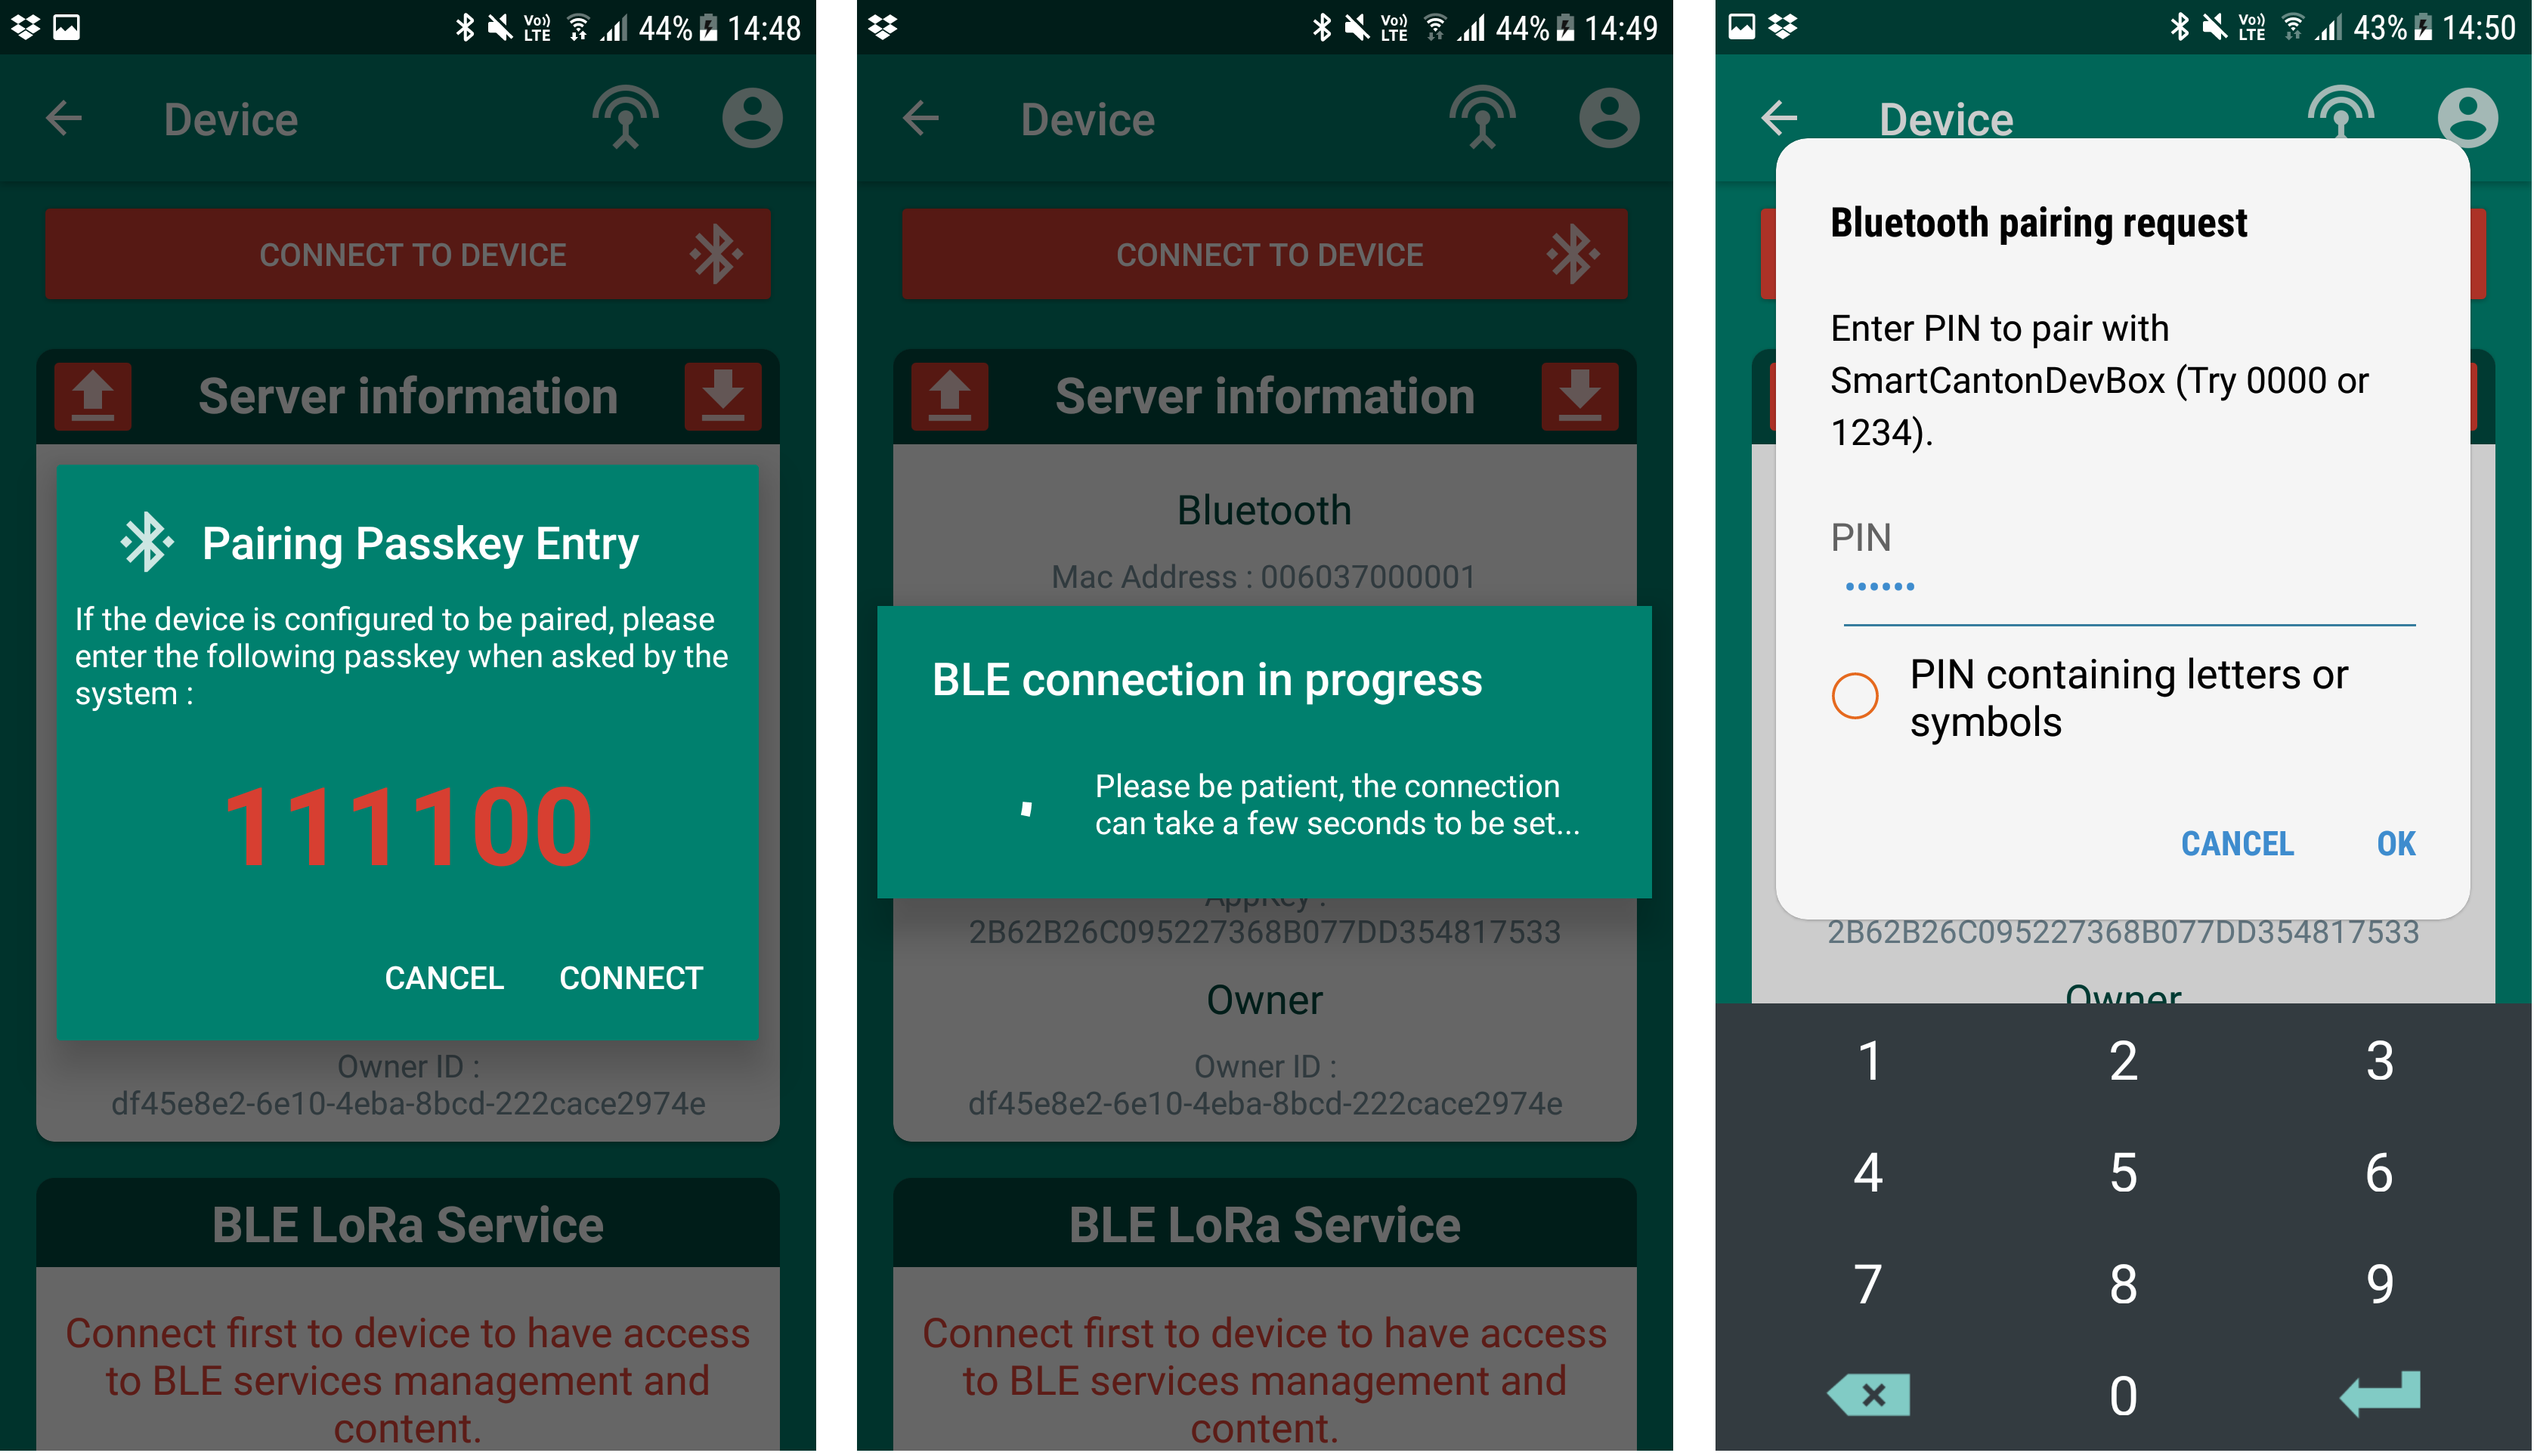
\includegraphics[width=1.0\textwidth]{Figures/Appendixes/Android/ble_dev_connection_process.png}
    \caption{SmartCanton Manager connection progress}
    \label{fig_apdx-ble_dev_connection_process}
\end{figure}

To connect to the device using Bluetooth Low Energy, the red button named \texttt{CONNECT TO DEVICE} on the top of the fragment needs to be pressed. The \cref{fig_apdx-ble_dev_connected_startup} shows the sequence of the connection. First a dialog inform the user that a BLE Passkey is present in the device and that the user need to remember it. Then the application will try to connect to the device. Finally, Android will ask the user to pair and bond with the device using the BLE Passkey previously displayed.


\begin{figure}[ht!]
    \centering
    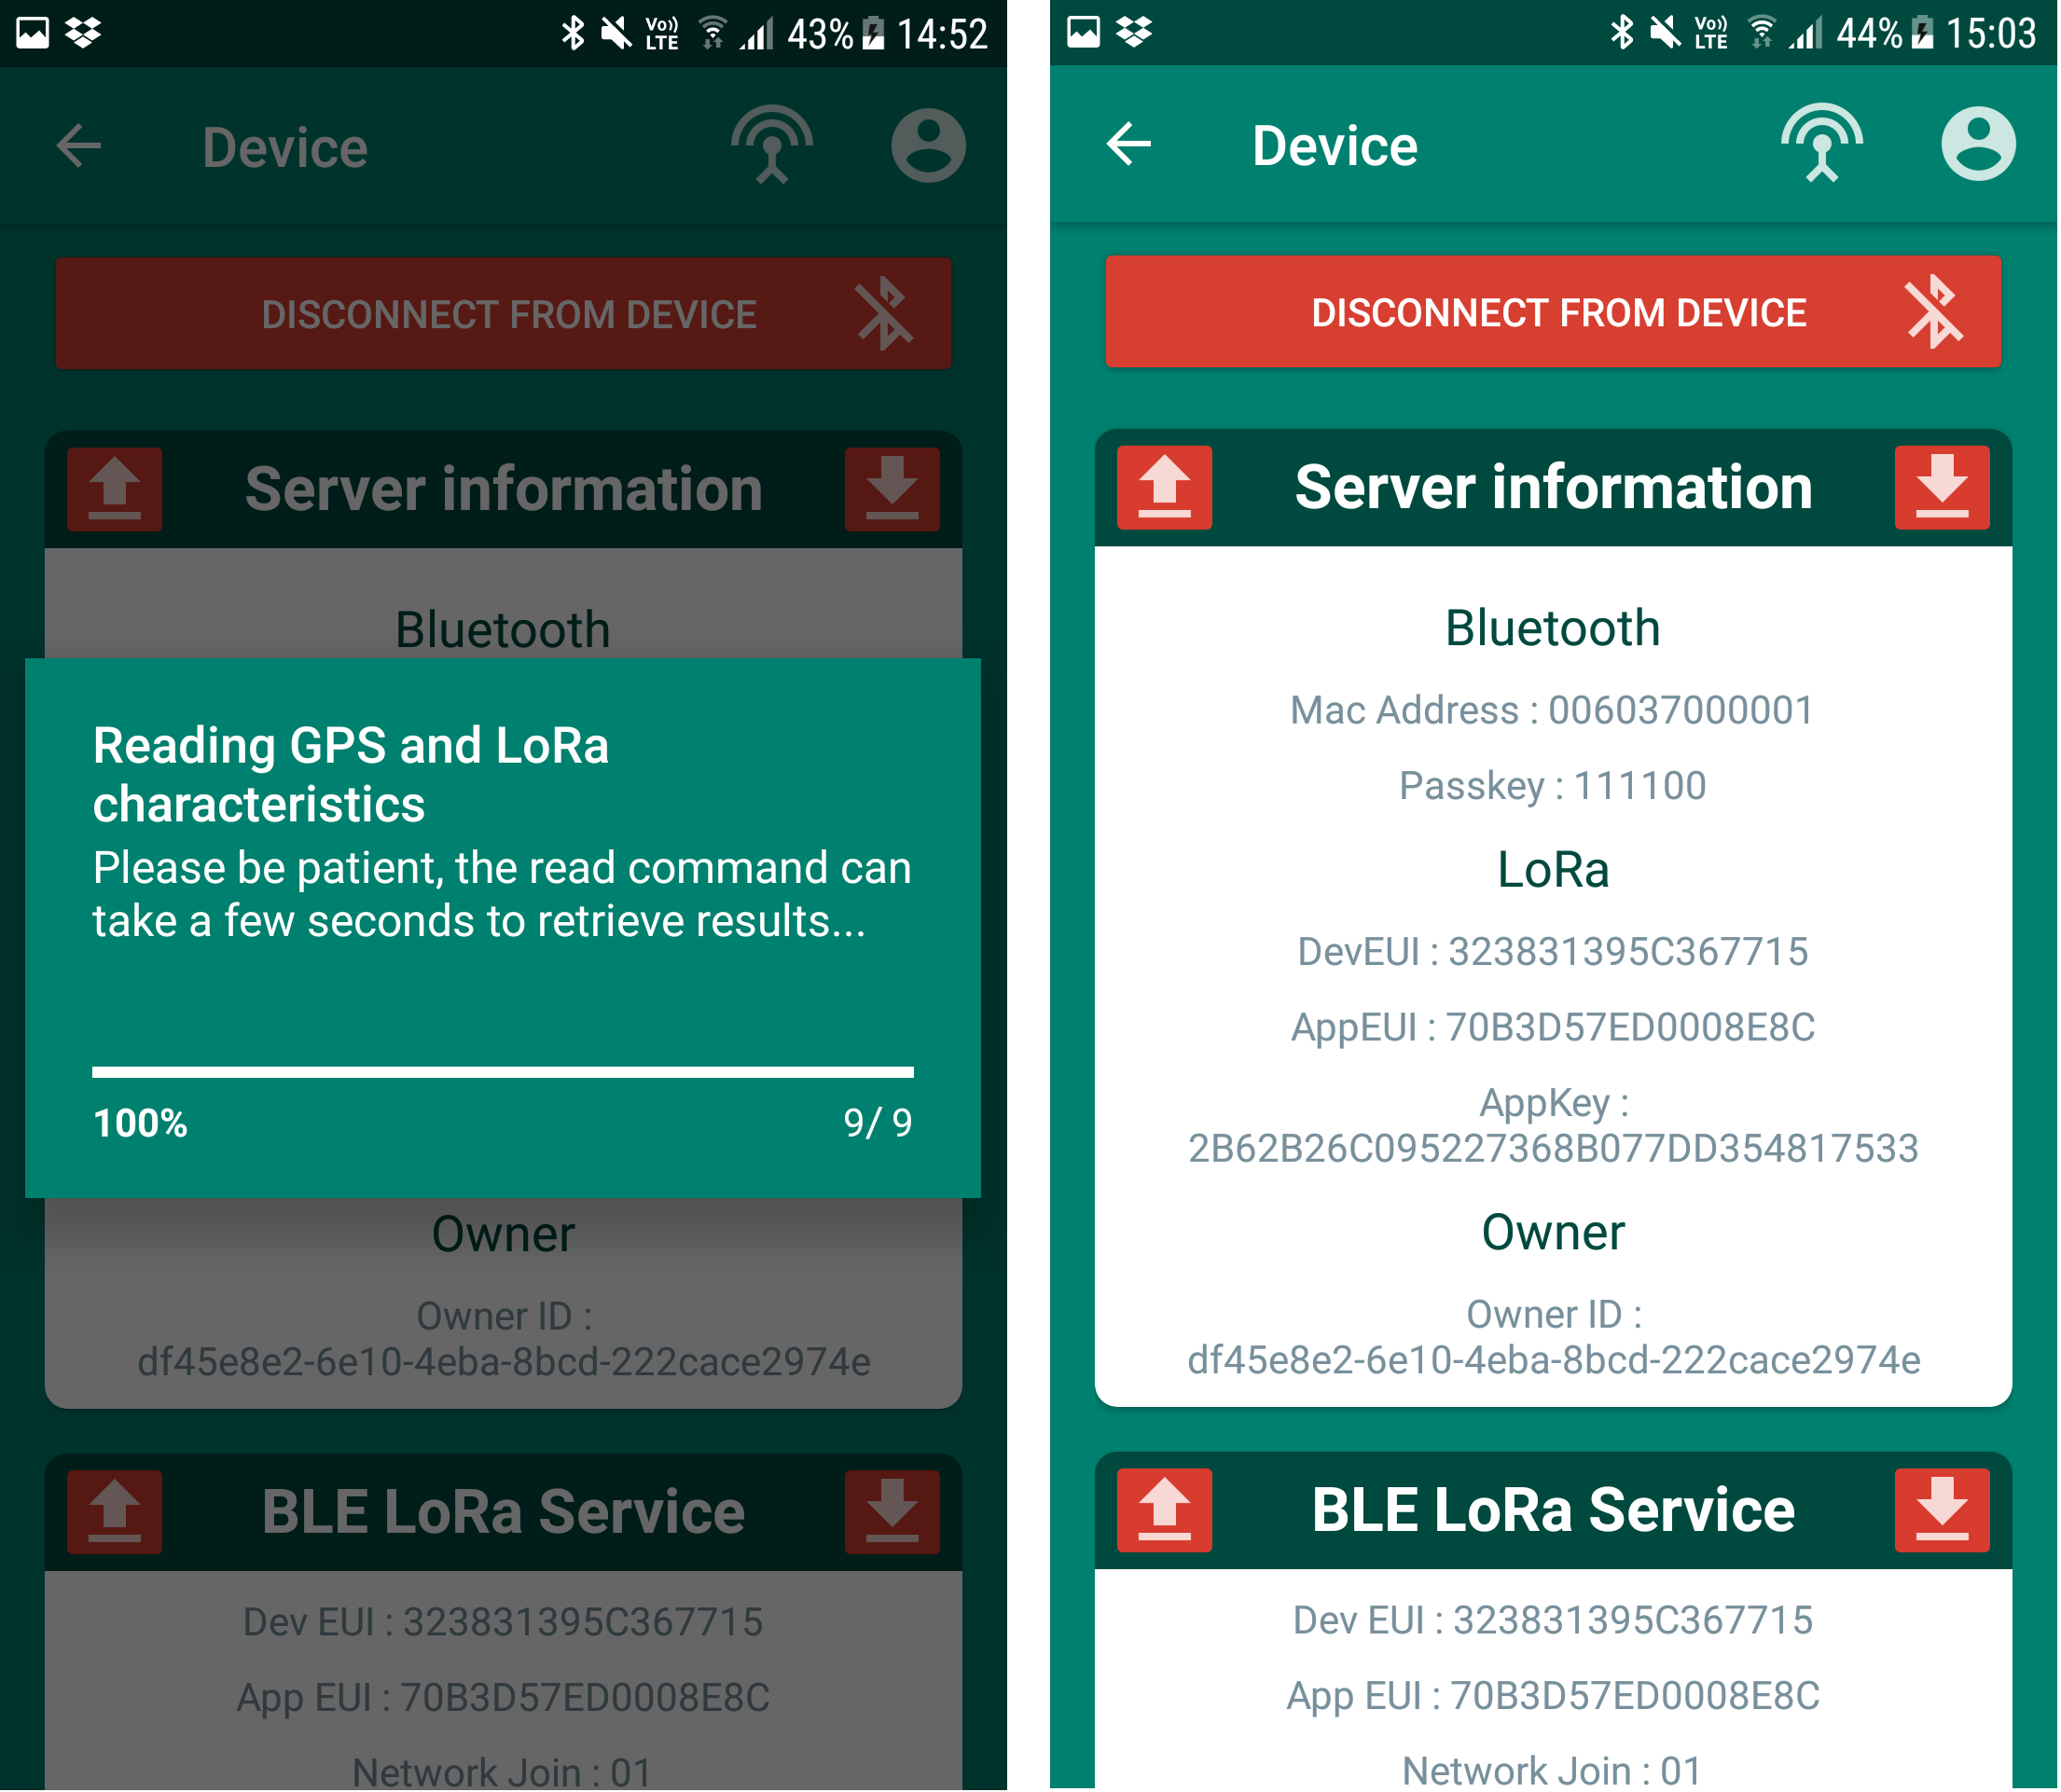
\includegraphics[width=0.66\textwidth]{Figures/Appendixes/Android/ble_dev_connected_startup.png}
    \caption{SmartCanton Manager device connected and characteristics read}
    \label{fig_apdx-ble_dev_connected_startup}
\end{figure}

Once the device is connected, the characteristics from the LoRa Service and the GPS of the DevBox are read and displayed in their respective cards, as shown on the \cref{fig_apdx-ble_dev_connected_startup}. The user can access to the multiples Bluetooth services available on the device. The user can disconnect from the device by leaving the current fragment (back button) or by pressing the \texttt{DISCONNECT FROM DEVICE} button on the top of the page.

\begin{figure}[ht!]
    \centering
    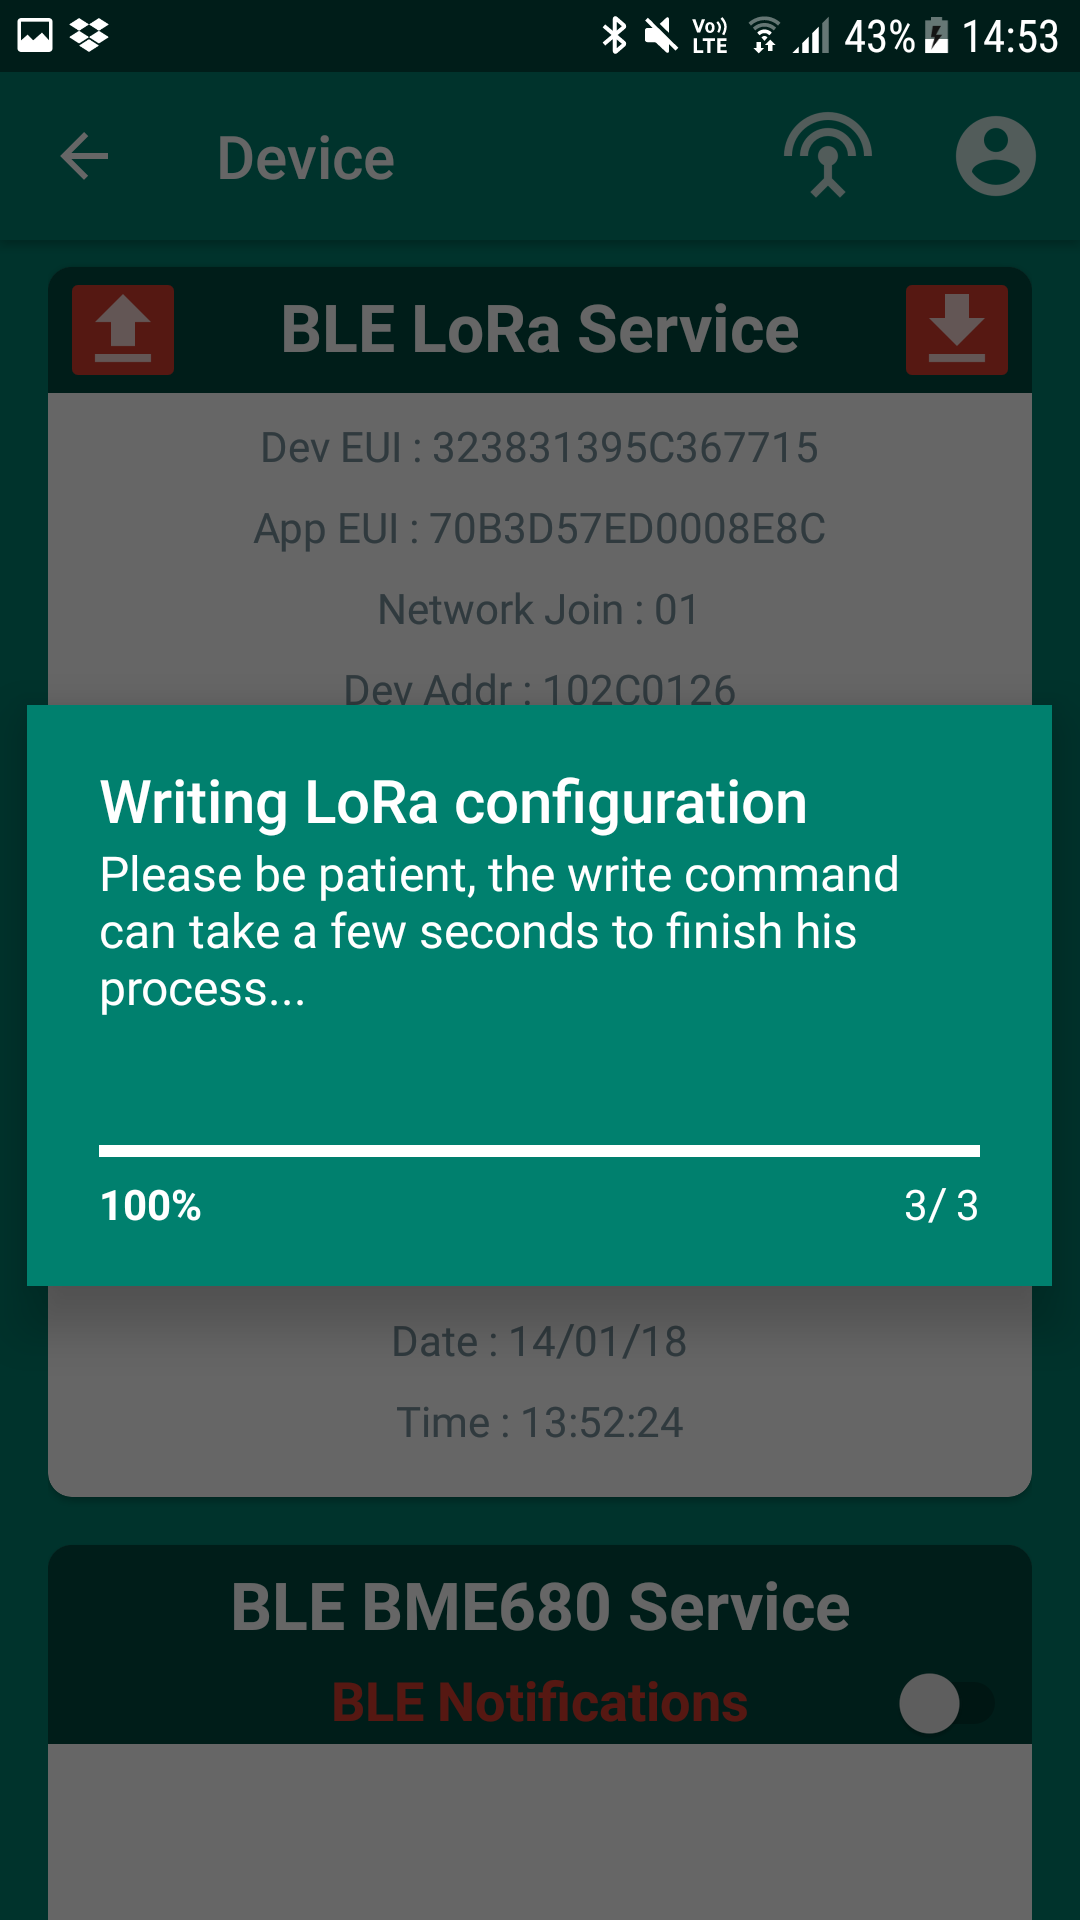
\includegraphics[width=0.33\textwidth]{Figures/Appendixes/Android/ble_dev_writing_lora_new_config.png}
    \caption{SmartCanton Manager update LoRaWAN config from server configuration}
    \label{fig_apdx-ble_dev_writing_lora_new_config}
\end{figure}

When the red arrow on the left of the \texttt{BLE LoRaWAN Service} is pressed, the device will be configured with the data read from the Server and diplayed in the \texttt{Server information} card. While the LoRaWAN service is been updated, a progress dialog is shown like in the \cref{fig_apdx-ble_dev_writing_lora_new_config}.

\begin{figure}[ht!]
    \centering
    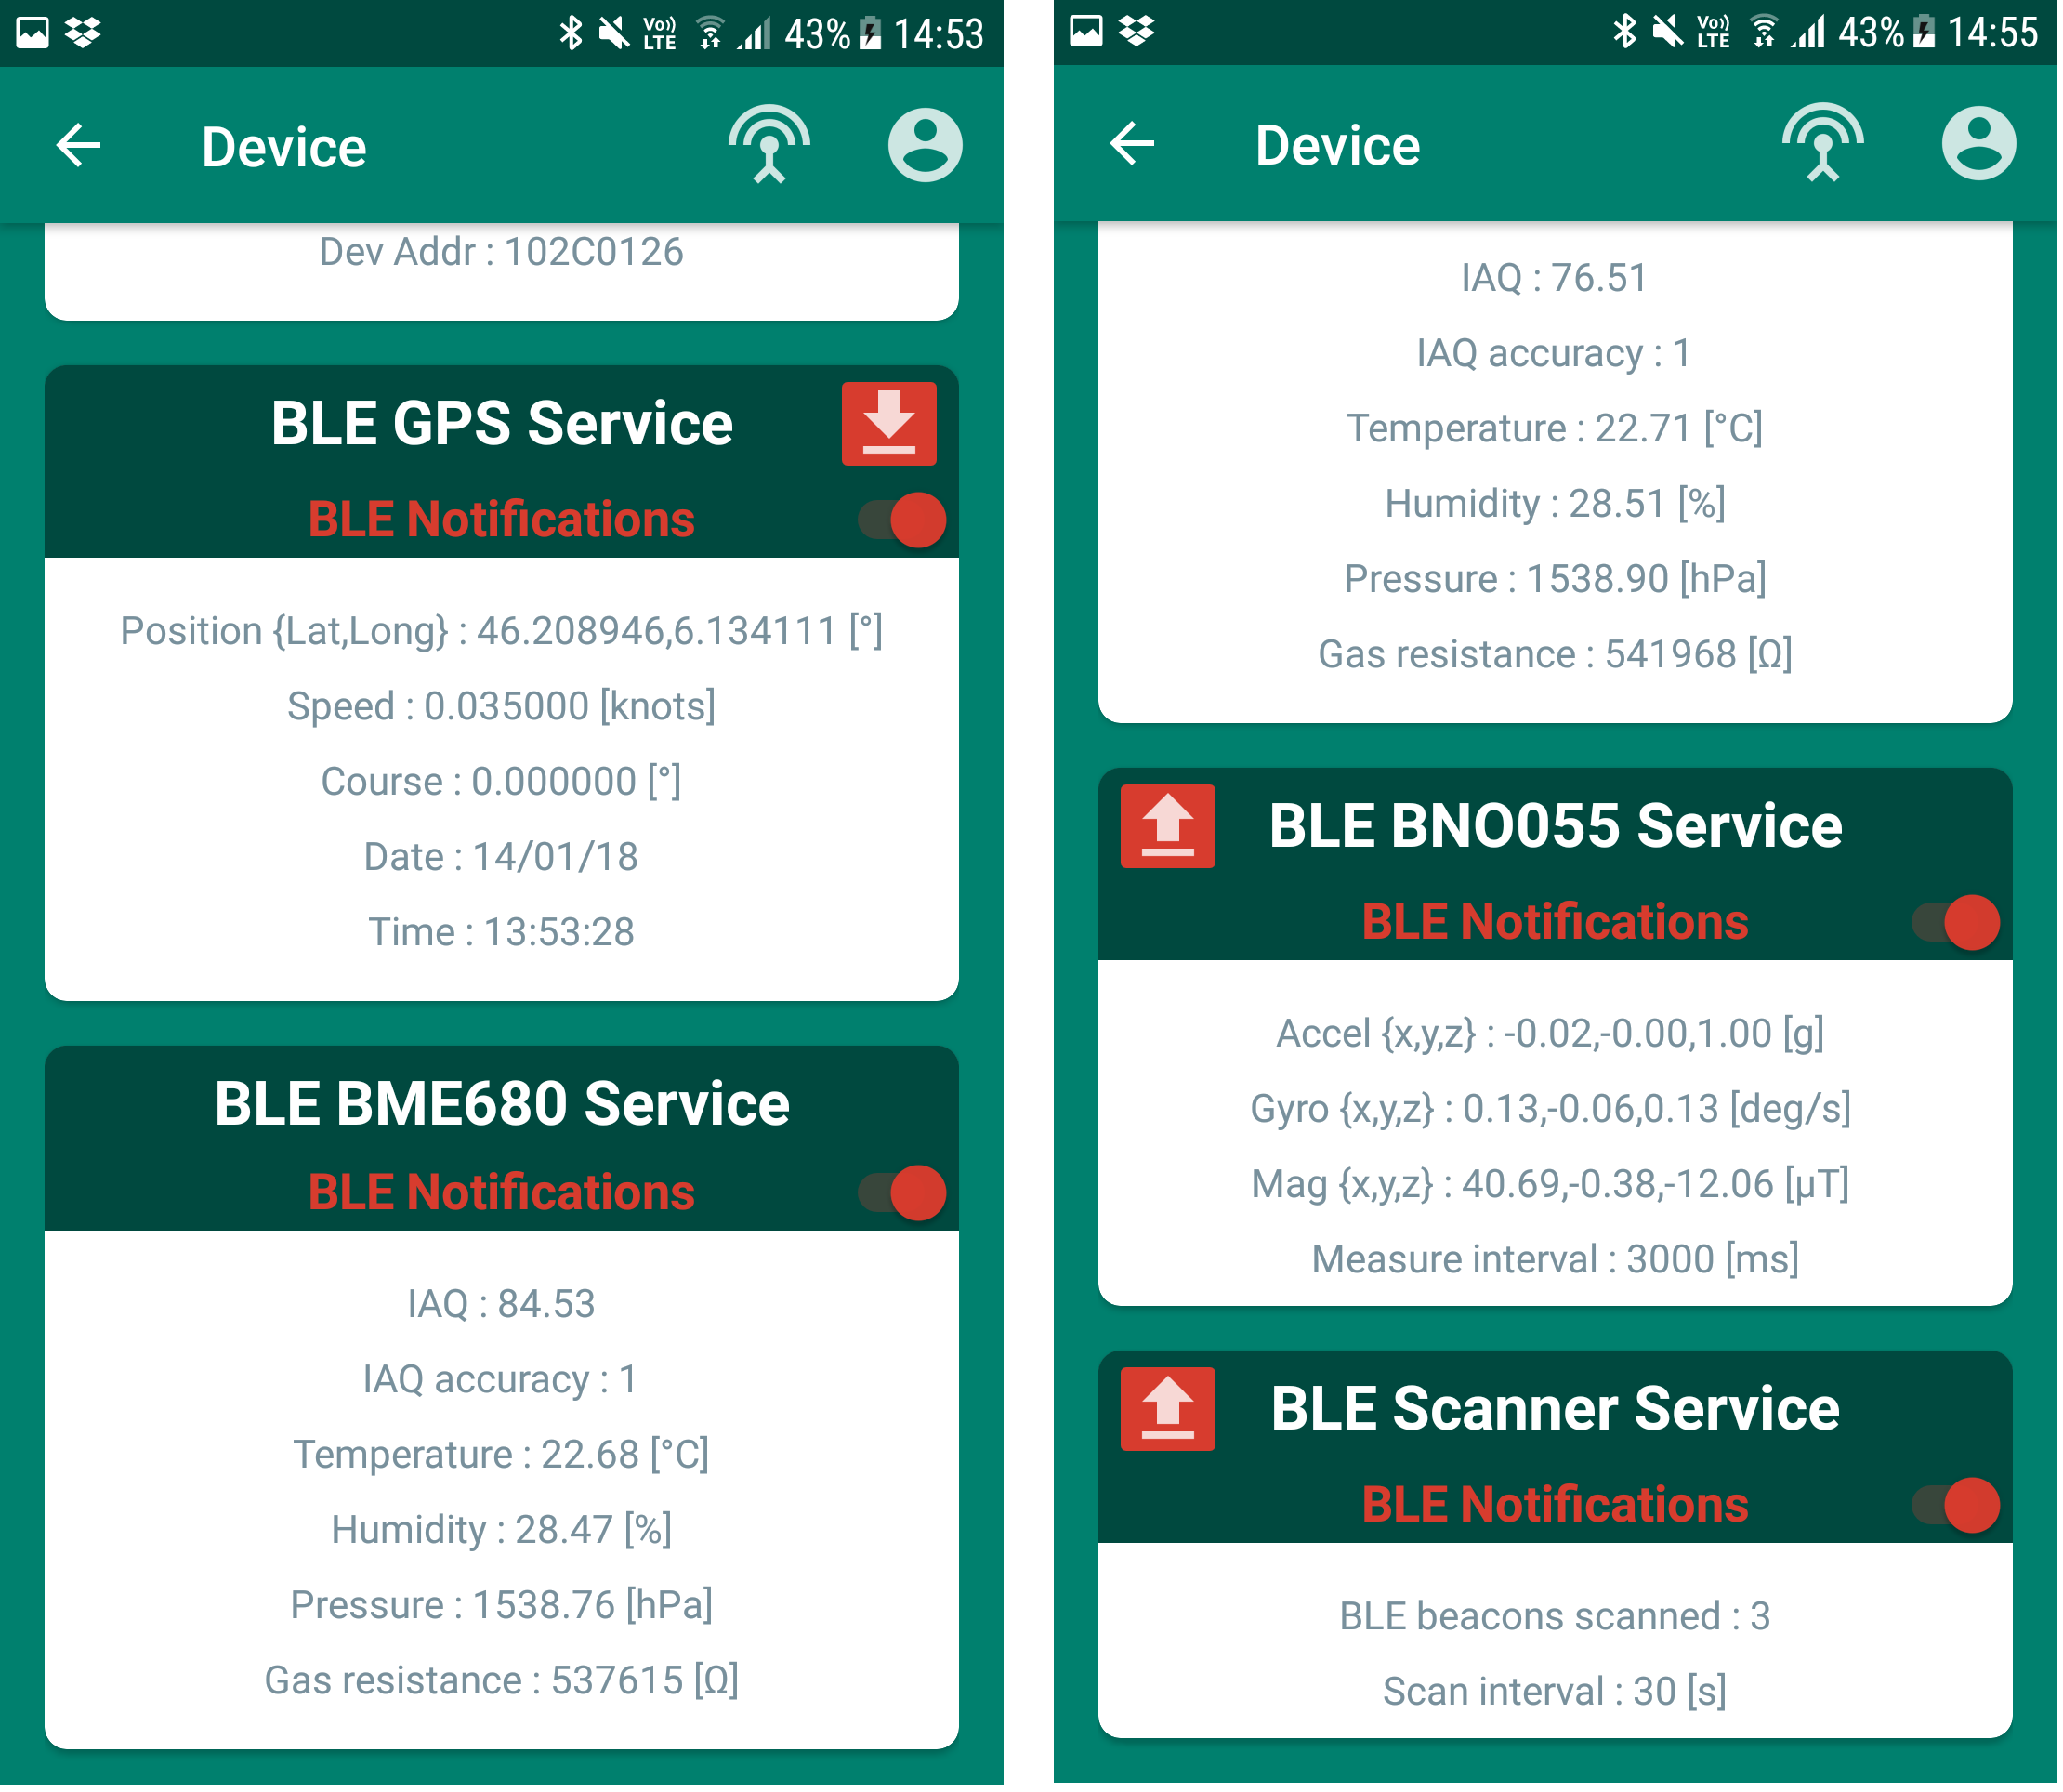
\includegraphics[width=0.66\textwidth]{Figures/Appendixes/Android/ble_dev_en_notif.png}
    \caption{SmartCanton Manager enable sensors notifications}
    \label{fig_apdx-ble_dev_en_notif}
\end{figure}


The user can toggle the notifications button for each sensor, as shown by the \cref{fig_apdx-ble_dev_en_notif}. Everytime a new data is read from the sensors, the application will display it.

\begin{figure}[ht!]
    \centering
    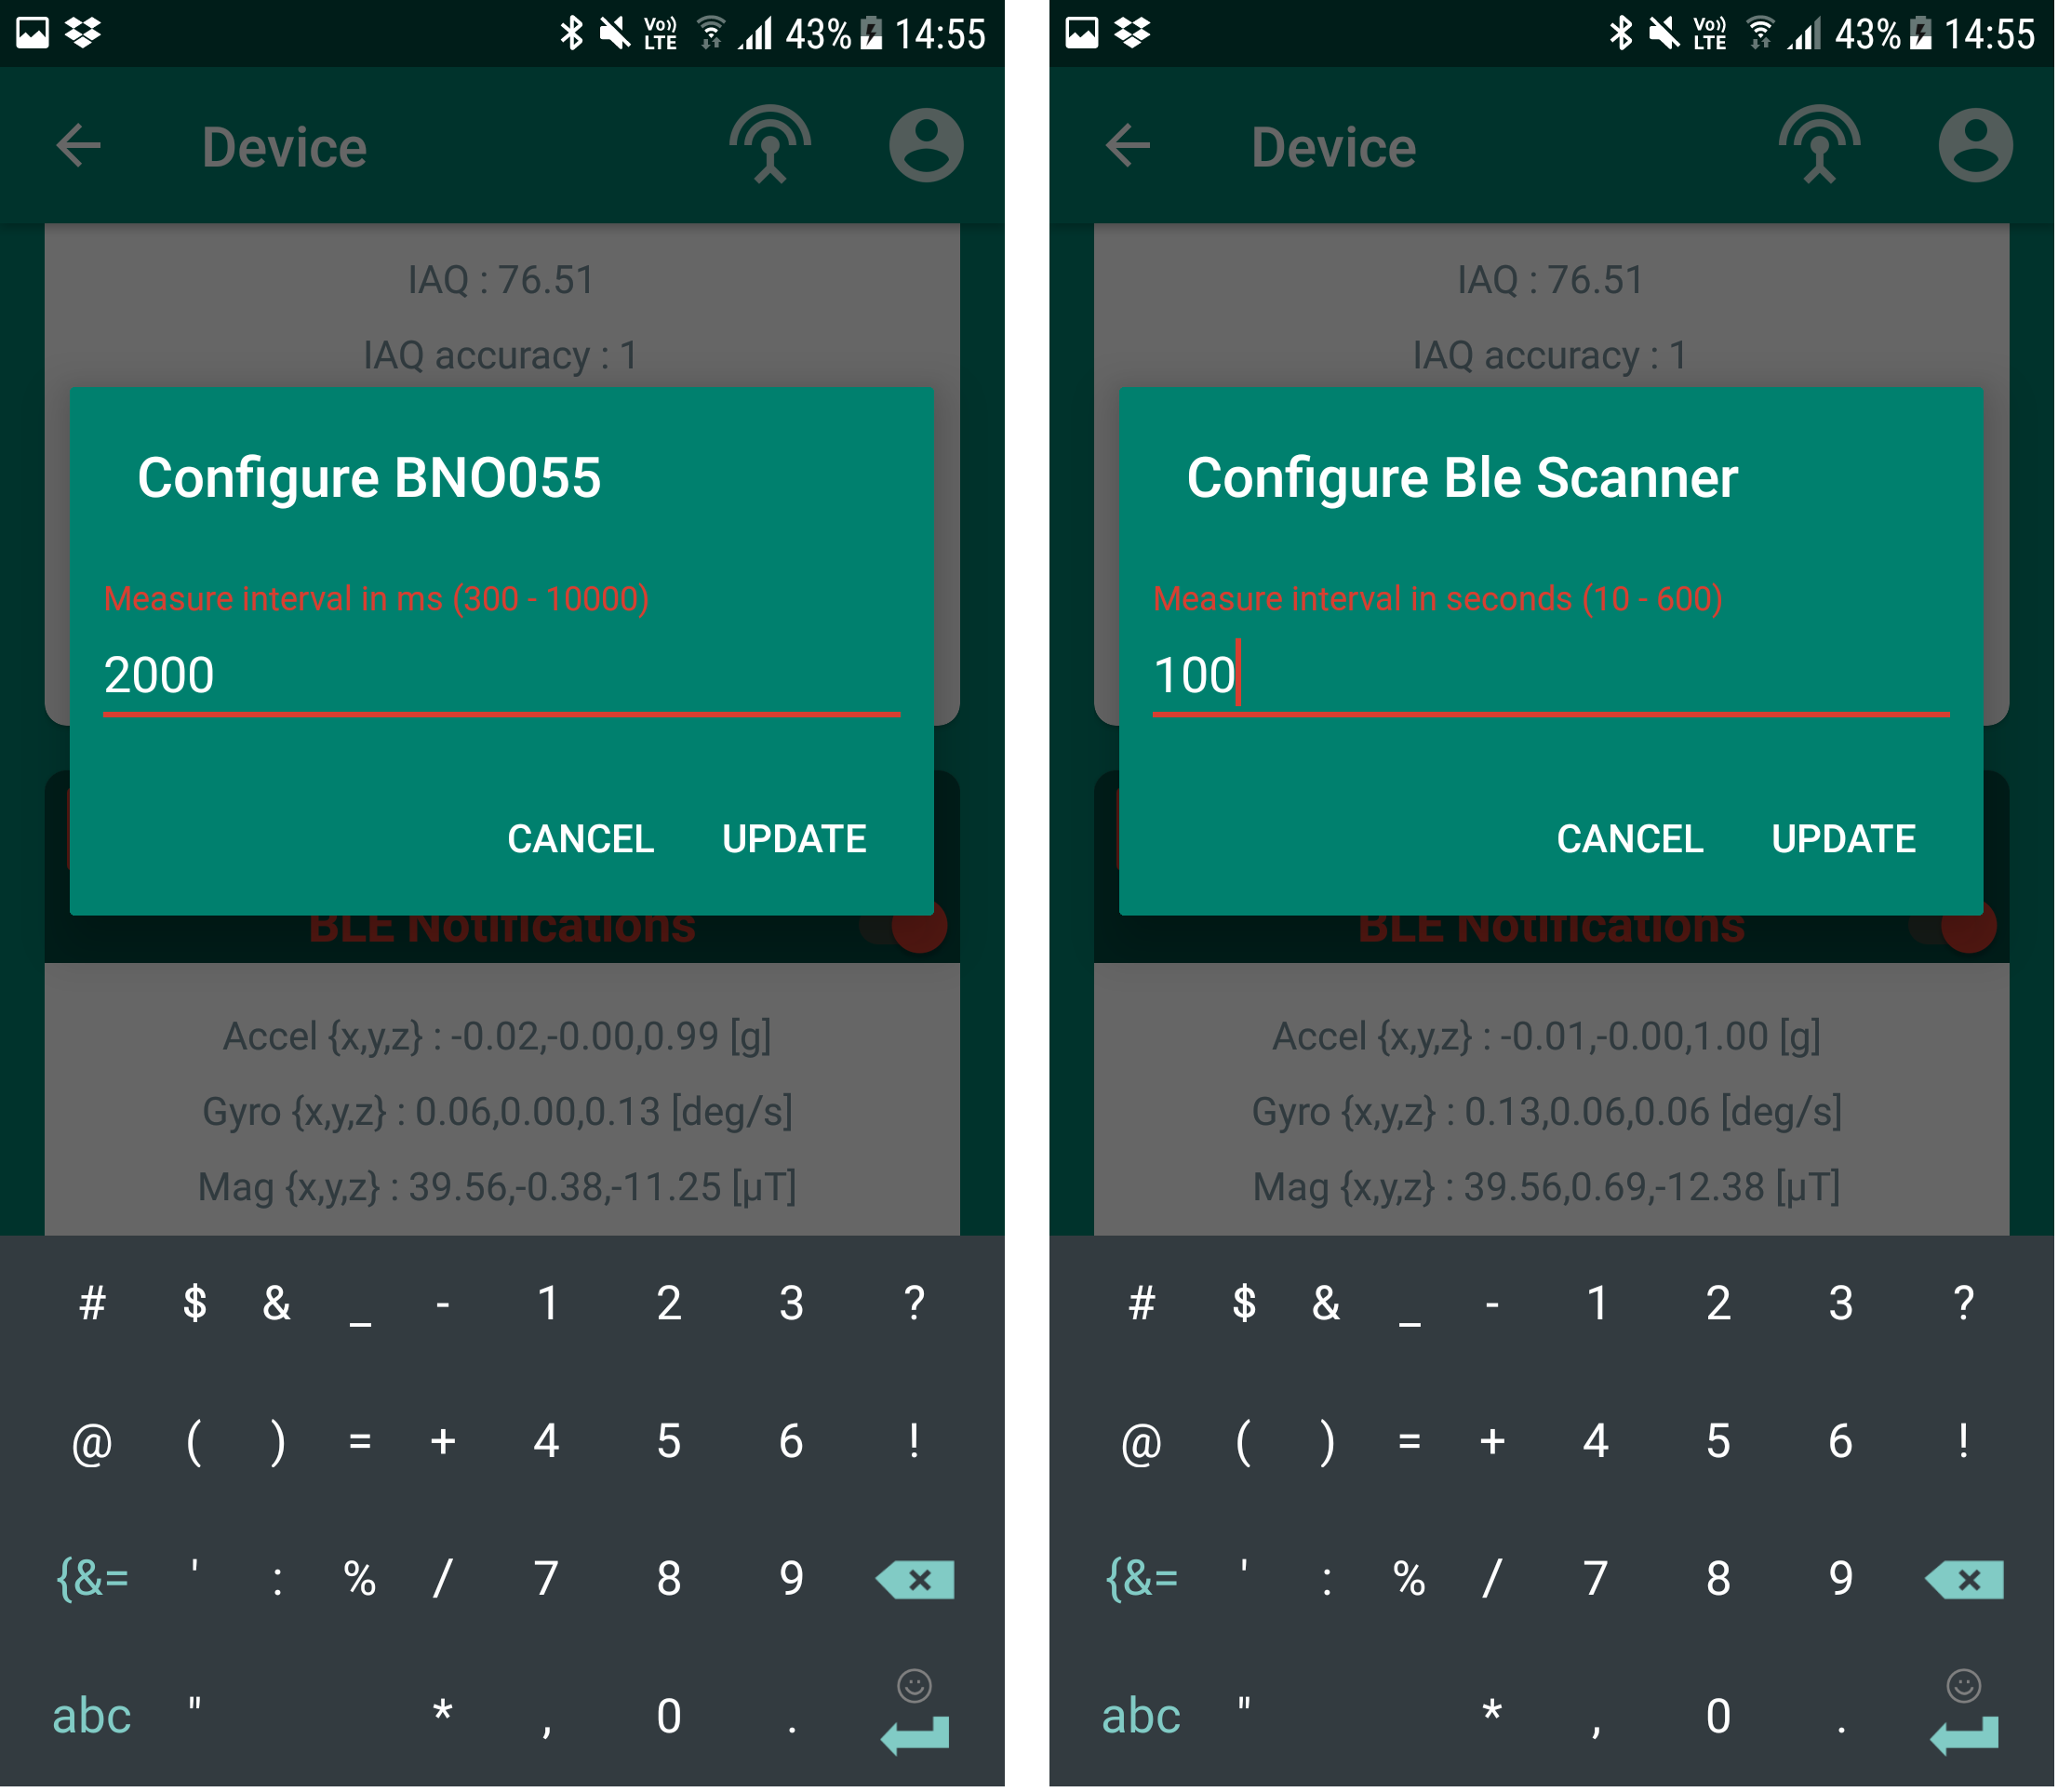
\includegraphics[width=0.66\textwidth]{Figures/Appendixes/Android/ble_dev_change_bno055_orblescan_config.png}
    \caption{SmartCanton Manager edit bno055 or ble scanner interval}
    \label{fig_apdx-ble_dev_change_bno055_orblescan_config}
\end{figure}
The user can configure the interval beetween each notifications from the BNO055 or the BLE Scanner, as shown by the \cref{fig_apdx-ble_dev_change_bno055_orblescan_config}.

% ---------------------------------------------------------------------- %
\FloatBarrier
\section{Profile Activity}
% ---------------------------------------------------------------------- %
\begin{figure}[ht!]
    \centering
    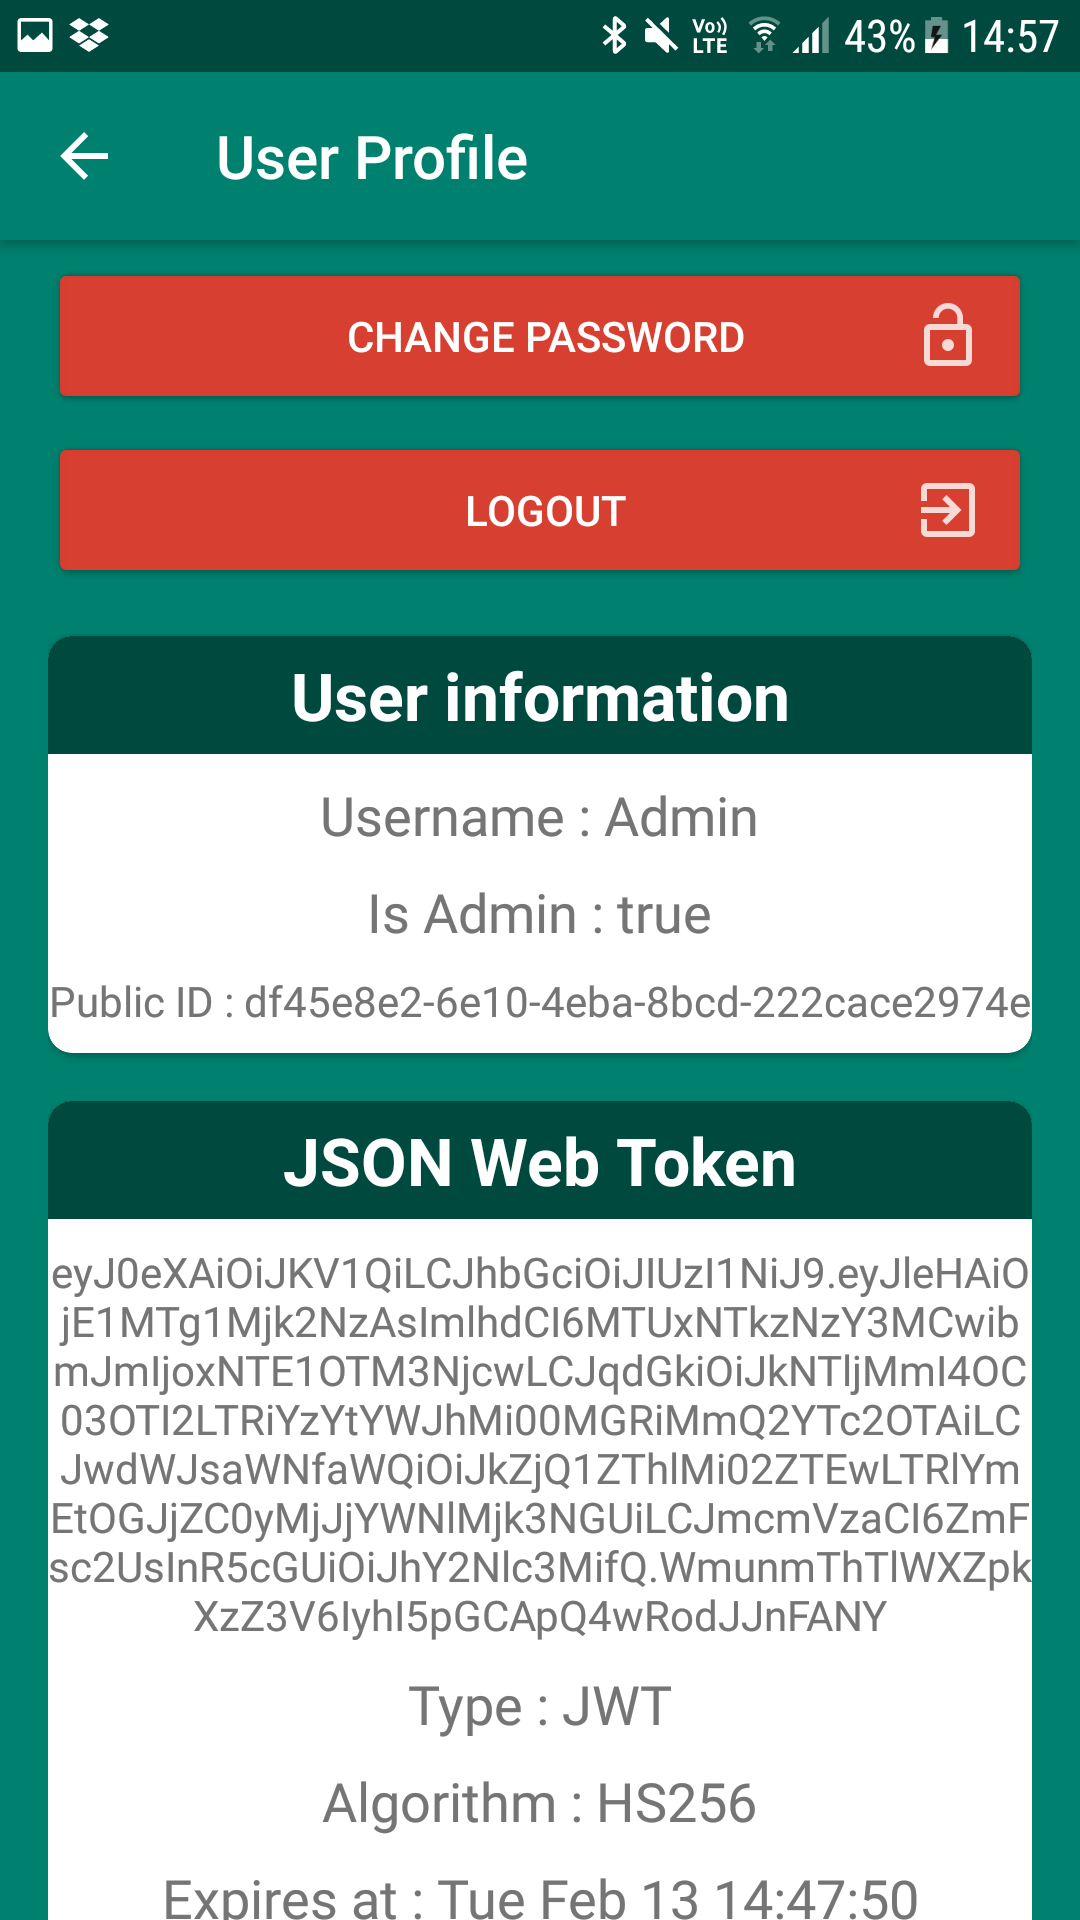
\includegraphics[width=0.33\textwidth]{Figures/Appendixes/Android/profile_activity.png}
    \caption{SmartCanton Manager profile activity}
    \label{fig_apdx-profile_activity}
\end{figure}

The user can access his profile by clicking on the user icon on the Action Bar. The profile activity, as it can be seen on the \cref{fig_apdx-profile_activity}, contain all information stored on the server for the current logged user. The user can logout from the current session by pressing the \texttt{LOGOUT} button.\\

% ---------------------------------------------------------------------- %
\FloatBarrier
\section{Beacon Generator Activity}
% ---------------------------------------------------------------------- %
\begin{figure}[ht!]
    \centering
    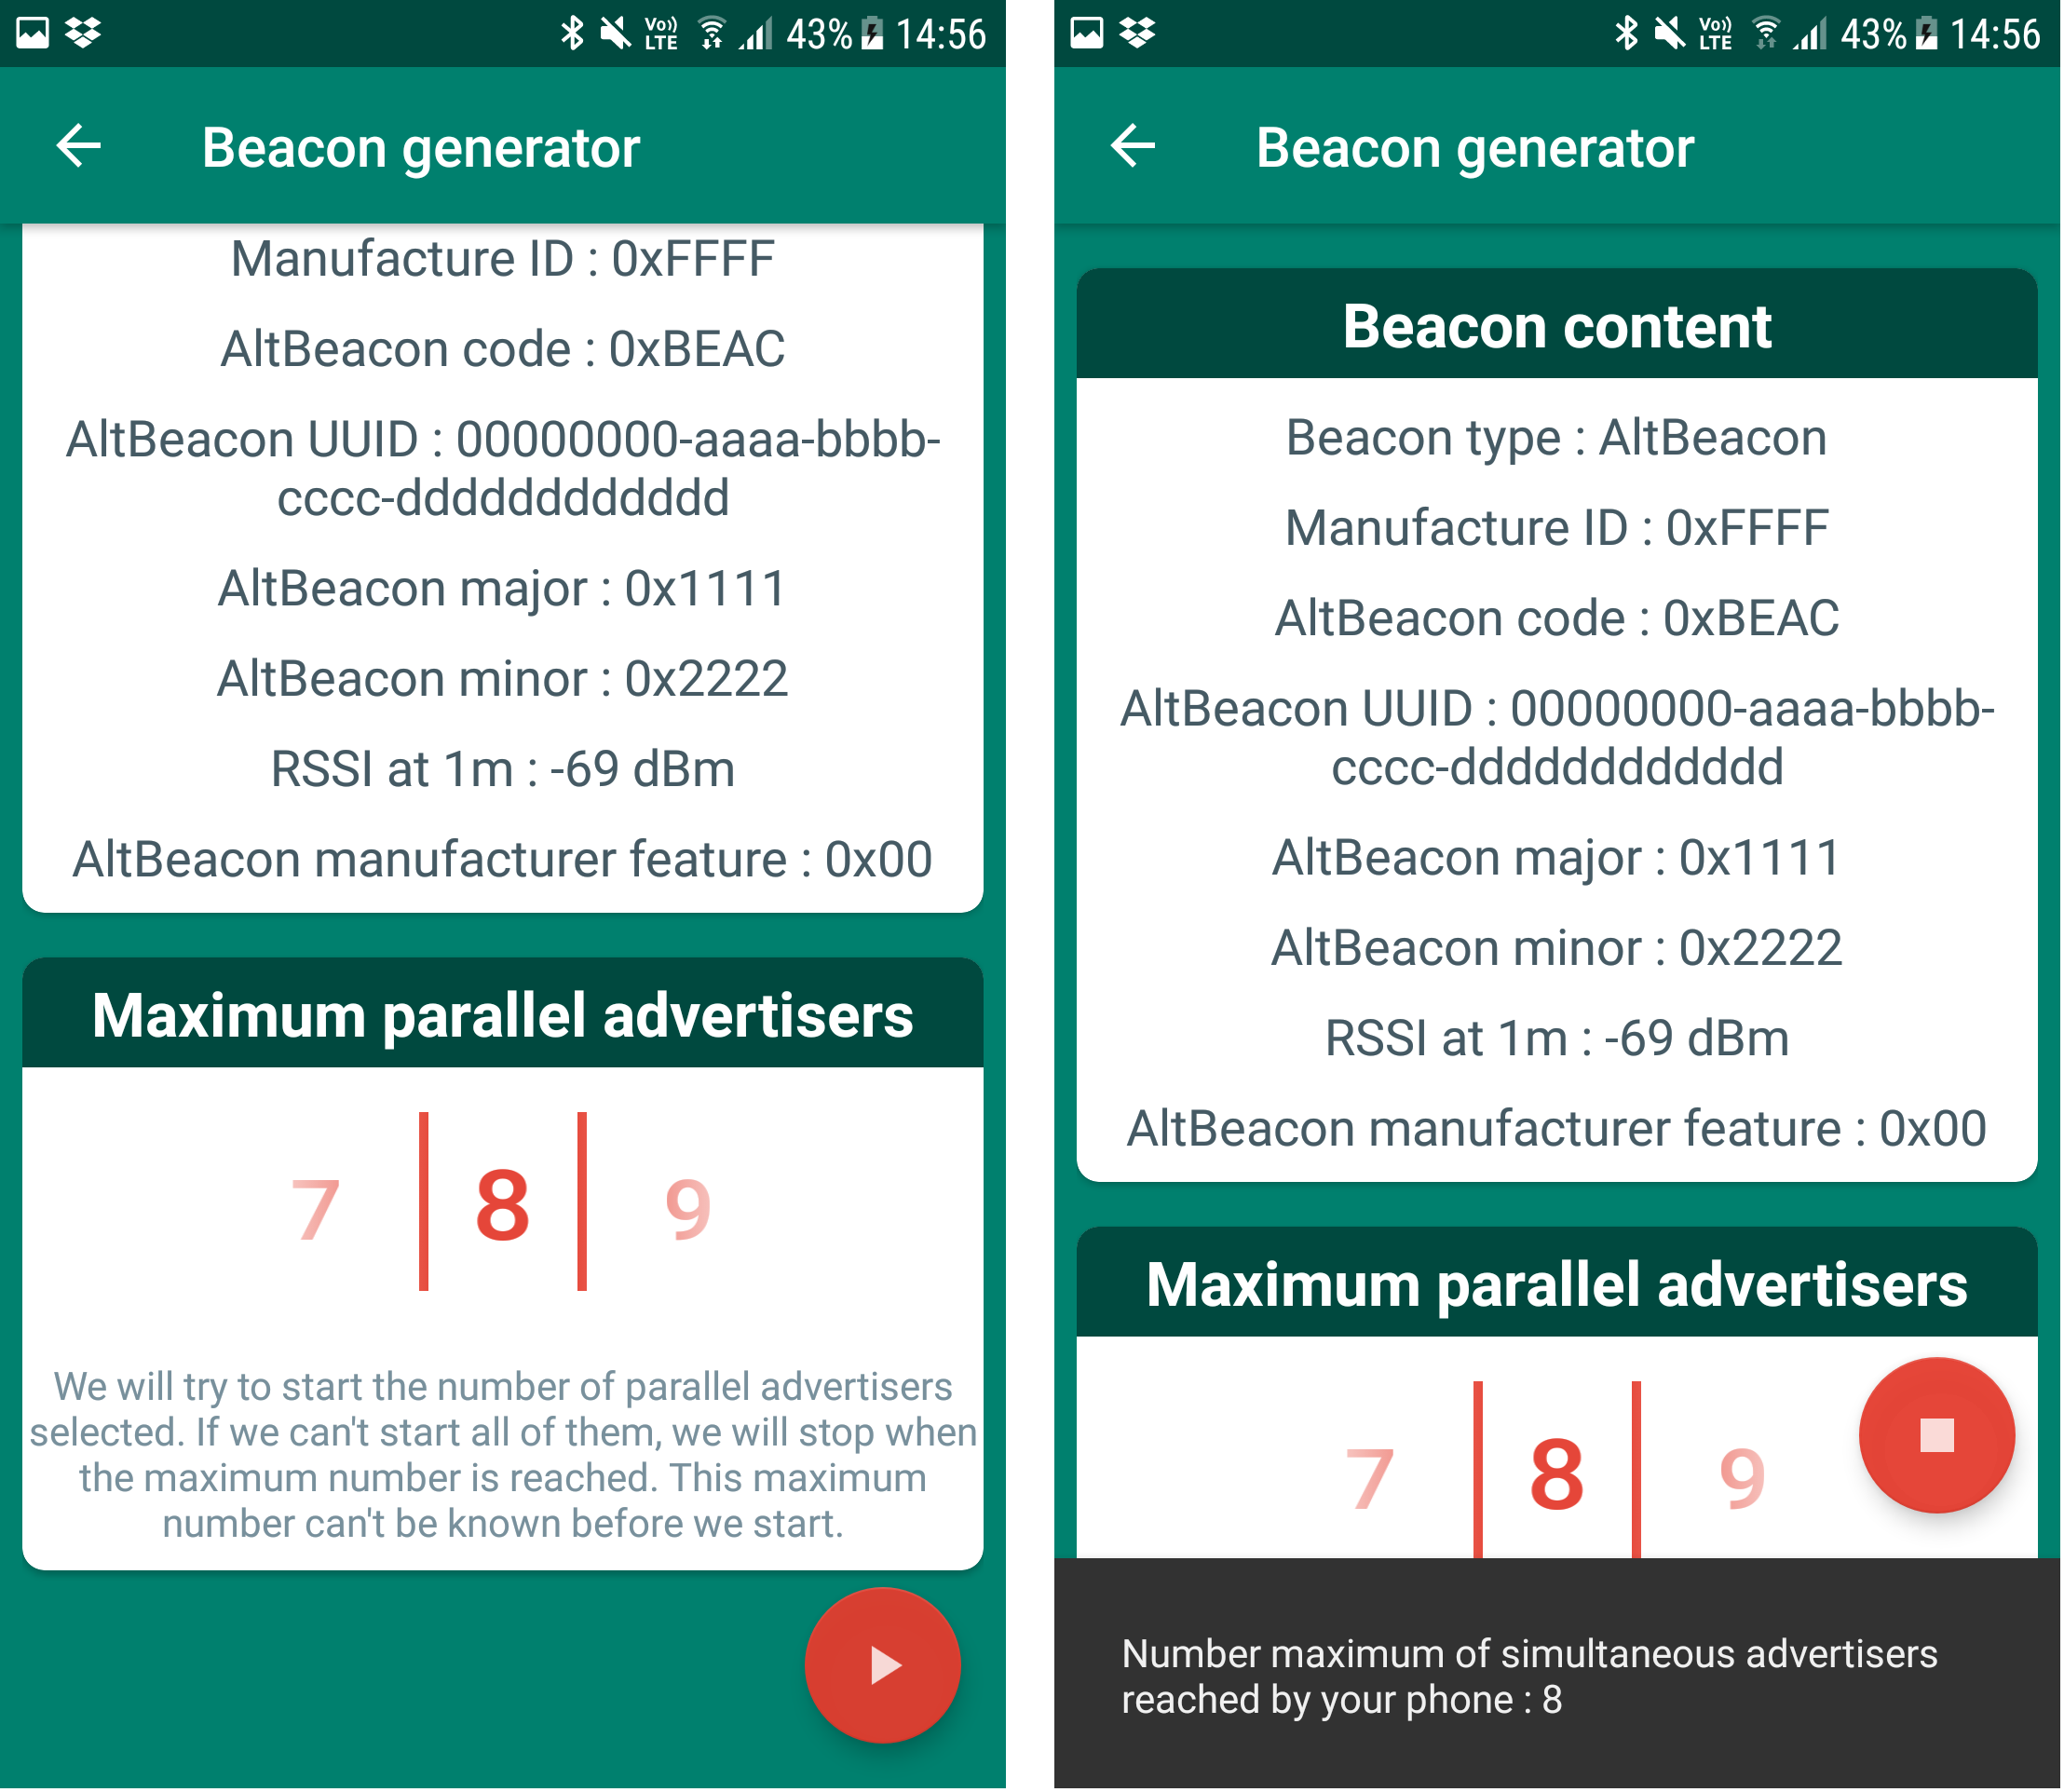
\includegraphics[width=0.66\textwidth]{Figures/Appendixes/Android/beacon_gen_activity_start_adv.png}
    \caption{SmartCanton Manager beacon generator activity}
    \label{fig_apdx-beacon_gen_activity_start_adv}
\end{figure}
\FloatBarrier

A beacon generator has been integrated inside the Android application. His purpose is to simulate nearby devices that can be scanned by a DevBox. The \cref{fig_apdx-beacon_gen_activity_start_adv} show the activity layout and how the app react when the \textit{play} button is pressed.

The user can select the number of devices that will be simulated by the application. However, each device has a number of maximum advertiser that can run at the same time. If the user select a number of devices greater than the maximum number available, the maximum number will be displayed to the user, as shown by the \cref{fig_apdx-beacon_gen_activity_start_adv}.